\documentclass[10pt]{article}
\usepackage{icmlko}

\icmlmeta{IP 파운데이션 월드모델}{294}{세 번 건너 봤다}{크로스 도메인 전이를 세 방법으로 시도했다 --- 표본이 처음으로 충분했던 세 번째에서도 건너오는 것이 문턱의 4분의 1이다}

\begin{document}

\twocolumn[
\icmlheader

\begin{abstract}
로드맵이 상태 층의 선결과제로 지목한 크로스 도메인 전이를 세 방법으로
시도했다. \textbf{① IP 그래프}(노트 291) --- 이미 있는
\texttt{ip\_graph.json} 이 lab 의 세 도메인과 붙지만 다른 도메인의 더 이른
라벨을 가진 유보 행이 \textbf{2개}다. \textbf{② 만화 별칭}(노트 293) ---
\texttt{cache\_manga\_kr} 의 한글 원제로 만화↔웹툰이 1 $\to$ 175건이 되는데
152건이 \emph{같은 작품}이고 시간 인과가 서는 것은 \textbf{23건(0.8\%)},
그마저 lab 의 만화 도메인(JP 전용)에는 없다. \textbf{③ 회사 이력}(이 노트)
--- 게임과 모바일이 회사 \textbf{64개}로 겹치고 \textbf{게임 레코드의 49\%}를
건드린다. 시간 인과도 선다(그 출시일 이전 것만 센다). 라벨도 안 본다.
\textbf{표본이 처음으로 충분했다.} 그리고 게임은 짝SE 0.0074 로 판에서
검출 문턱이 제일 낮다(0.015). 쟀다 --- \textbf{학습 구간 상관은 오른다}
($+$0.2002 $\to$ $+$0.2149) 그리고 \textbf{유보 이득은 게임 $+$0.0040 ·
모바일 $-$0.0019}, 판 $+$0.0008, 진짜 0개. \textbf{문턱의 4분의 1이다.}
세 번 다 못 잰 것이 아니다 --- 앞의 둘은 \emph{표본이 없어서} 못 쟀고,
이번은 \textbf{표본이 있는데 효과가 작다.} 그게 다른 답이다.
\textbf{건널 다리가 생겨도 건너오는 것이 작다.}
\end{abstract}
]

\section{세 번째 시도는 표본이 있었다}

앞의 두 시도는 표본에서 막혔다.

\begin{center}\small
\begin{tabular}{lrl}
\hline
시도 & 닿는 행 & 막힌 곳 \\
\hline
IP 그래프(291) & 2 & 유보 2행 --- 못 잰다 \\
만화 별칭(293) & 0.8\% & 152/175 가 같은 작품 \\
\textbf{회사 이력(294)} & \textbf{49\%} & --- \\
\hline
\end{tabular}
\end{center}

회사는 다르다. 게임의 \texttt{developers}/\texttt{publishers} 와 모바일의
\texttt{artist} 를 법인 접미어(Co./Ltd./Inc./Games/Studio$\ldots$)를 걷고
맞추면 \textbf{64개가 겹치고} 게임 482건 중 \textbf{234건(49\%)} · 모바일
2,000건 중 160건이 그 회사들의 것이다(CAPCOM · 반다이남코 · KONAMI ·
네오위즈 · 넷마블 · Ubisoft $\ldots$).

\paragraph{그리고 회사는 쓸 수 있는 종류다} 노트 293이 만화 라벨을 못 쓴다고
한 이유가 ``지금 긁은 스냅샷''이었는데, \textbf{회사 정체는 출시 시점에
확정}이다. 세는 것도 \textbf{그 출시일 이전 것만} 센다 --- 시간 인과가 선다.
라벨도 한 번도 안 본다.

\paragraph{물음이 깨끗하다} 두 도메인은 \emph{이미} \texttt{venue\_prominence}
를 ``창작자의 사전 작품 수''로 채우는데 \textbf{도메인 안에서만} 센다.
\textbf{가로질러 세면 나아지나?}

\section{학습에서는 오르고 유보에서는 안 온다}

\begin{figure*}[t]
\centering
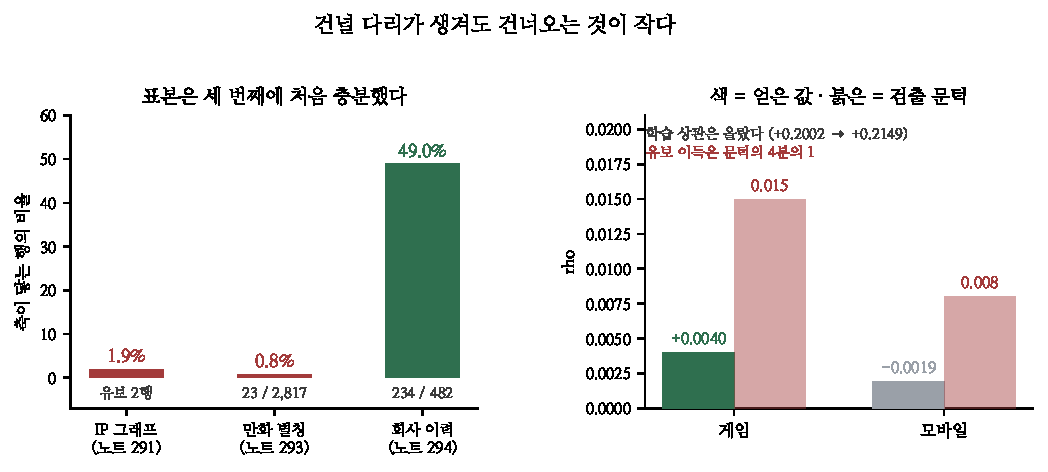
\includegraphics[width=\textwidth]{figs/three.pdf}
\caption{왼쪽 --- 세 시도가 닿는 행의 비율. 오른쪽 --- 회사 이력을 가로질러
셌을 때의 유보 이득과 그 도메인의 검출 문턱(노트 274).}
\end{figure*}

\begin{center}\footnotesize
\begin{tabular}{lrr}
\hline
& 게임 & 모바일 \\
\hline
값이 커지는 행 & 137/482 (28\%) & 51/2000 (3\%) \\
평균 & 1.61 $\to$ 2.48 & 1.10 $\to$ 1.15 \\
\textbf{학습 상관} & \textbf{$+$0.2002 $\to$ $+$0.2149} & $+$0.1330 $\to$ $+$0.1380 \\
\hline
유보 $\rho$ & 0.6158 $\to$ 0.6198 & 0.5510 $\to$ 0.5491 \\
\textbf{이득} & \textbf{$+$0.0040} & $-$0.0019 \\
검출 문턱 & 0.015 & 0.008 \\
\hline
판 & \multicolumn{2}{c}{0.4819 $\to$ 0.4827 ($+$0.0008) · 진짜 0개} \\
\hline
\end{tabular}
\end{center}

\textbf{학습 구간에서는 오른다.} 노트 239 · 285의 규약대로 채택 근거는 학습
구간이고 거기서 $+$0.2002 $\to$ $+$0.2149 다. \textbf{유보에서는 게임
$+$0.0040 --- 그 도메인 검출 문턱의 4분의 1}이다.

\paragraph{이번엔 ``못 쟀다''가 아니다} 오늘 여러 번 ``문턱 아래라 못 잰다''로
끝났는데(노트 282 아이돌 · 285 범주 · 287 넓힌 팝업 · 291 조인), 그때는
\emph{표본이 없어서} 문턱이 높았다. 여기는 다르다 --- 게임은 유보 180행에
짝SE 0.0074 로 \textbf{판에서 문턱이 제일 낮은 도메인}이고, 축이 49\% 를
건드리고, 그런데도 $+$0.0040 이다. \textbf{잴 수 있는 자에 대고 쟀더니 작았다.}

\paragraph{덤 --- 또 자리바꿈} 제일 크게 움직인 것이 \textbf{아이돌
$+$0.0493}($t{=}1.32$)인데 아이돌은 이 축의 마스크가 0 이다. 노트 259의
길이 다시 옮겨졌다. 유의하지 않다.

\section{그래서 크로스 도메인 갈래를 닫는다}

세 시도의 답이 서로 다르다.

\begin{center}\small
\begin{tabular}{lll}
\hline
시도 & 막힌 것 & 다음에 할 수 있는 것 \\
\hline
IP 그래프 & 표본(유보 2행) & 팝업 허브에서 늘리기 \\
만화 별칭 & 대상(같은 작품) & 없음 --- lab 이 이미 제외 \\
\textbf{회사 이력} & \textbf{효과 크기} & 다른 도메인 쌍 \\
\hline
\end{tabular}
\end{center}

\textbf{셋 중 둘은 기질이 없었고 하나는 기질이 있는데 신호가 작다.} 이것이
상태 층(블록 3)에 대해 이 실험실이 지금 말할 수 있는 것이다 --- 프롬프트 주입
세 번의 기각(B · B$'$ · B$''$)이 방법의 실패였는지 기질의 부재였는지 몰랐는데,
\textbf{적어도 lab 안에서는 기질이 거의 없다.}

\paragraph{남은 것}
\begin{center}\small
\begin{tabular}{ll}
\hline
갈래 & 왜 \\
\hline
하네스에서 재기 & MAPE 쪽은 분해능이 다르다 \\
팝업 허브 늘리기 & 노트 291의 조인은 여전히 유효 \\
회사 축을 남길까 & $+$0.0040 · 해 없음 · 학습 근거 있음 \\
KIOF 실측 & 여전히 Drive 에 문서 없음 \\
\hline
\end{tabular}
\end{center}

\paragraph{규약} \textbf{``못 쟀다''와 ``작았다''를 갈라 적는다.} 둘 다 진짜
0개로 끝나지만 다음 수가 다르다 --- 앞은 표본을 늘리면 되고 뒤는 그 길이
막힌 것이다. 오늘 넷이 앞이었고 이번이 처음 뒤다. 그리고 \textbf{제일 낮은
문턱을 가진 도메인에서 재라} --- 게임의 0.015 가 아니었으면 이번 것도
``못 쟀다''로 끝났을 것이고, 그러면 틀린 다음 수를 골랐을 것이다.

\end{document}
